\chapter[Motivation of the experiment]{Motivation of the experiment}
\label{chap:motivation}

The accelerating gradient profile in a travelling-wave cavity depends on the configuration of the electromagnetic field inside the cavity. The passage of the  beam modifies the internal field configuration. As a consequence, the gradient profile is modified and decreases along the structure.

At the same input power, the modification of the gradient profile is dependent on the beam current, as shown in Fig. \ref{grad_vs_I}. The result of the beam loading of the cavity is a reduction of the average accelerating gradient.

\begin{figure}[h]
\centering 
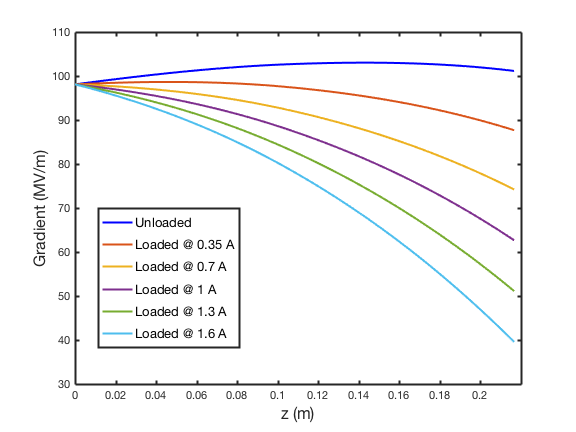
\includegraphics[scale=0.5]{pictures/Gradient_vs_current.png}
\caption{Gradient profile along the TD26CC structure at 43.3 MW input power. The unloaded case and the loaded with different current intensities are shown. The average gradient difference between the adjacent curves is approximately 5 MV/m.}
\label{grad_vs_I}
\end{figure}

\noindent
The particle energy gain is given by 
\begin{equation}
\Delta W  = q \int_0^L E_{\text{acc}} (z) \, dz = q \left \langle E_{\text{acc}} \right \rangle L
\label{en_gain}
\end{equation}
where q is the charge, E$_{\text{acc}}$ is the accelerating field and L the length of the accelerating structure.

Equation \ref{en_gain} shows that the energy gain is reduced when the accelerating cavity is loaded with the beam, compared to the unloaded condition. To compare the tests carried out without beam with the real running condition in an accelerator, it becomes necessary to raise the input power when the beam is present, in order to compensate for the reduction of average accelerating gradient. The nominal parameters for CLIC are 1.2 A of beam current and 100 MV/m of loaded accelerating gradient \cite{CLIC:cdr}. Figure \ref{100mvm} shows the variation of the gradient profile between loaded and unloaded running condition for the CLIC nominal operation. In this case the input power has to be raised from~43.3 MW to 61.3~MW to maintain the average accelerating gradient to 100 MV/m (see Table~\ref{TD26_param_1}).

\begin{figure}[h]
\centering 
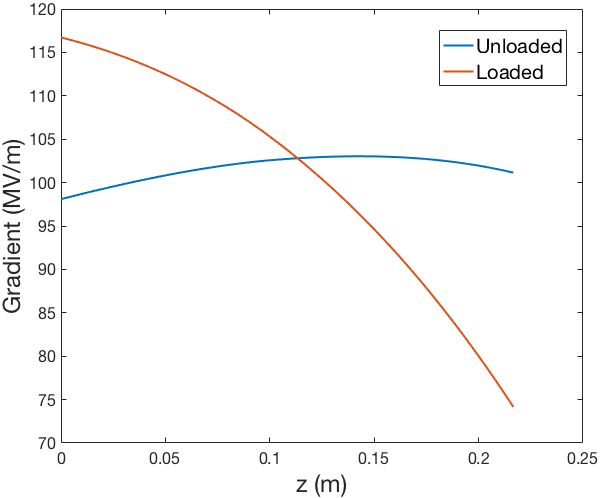
\includegraphics[scale=0.45]{pictures/grad_vs_IP.png}
\caption{Comparison of the loaded and unloaded gradient profile of the TD26CC structure loaded with the CLIC Main Beam. When loaded with a current of 1.2 A, the input power to maintain an average gradient of 100 MV/m passes from 43.3 MW in the unloaded case to 61.3 MW in the loaded case. }
\label{100mvm}
\end{figure}

All breakdown rate tests in literature have been conducted without  beam presence. Since the vacuum arc phenomenon is not described yet by a solid physical theory there is no way to predict a priori how the breakdown rate is affected by the presence of the beam. The first dedicated experiment and its results are described in this work.

The interesting measurements that can be carried out are:
\begin{enumerate}
\item Comparing  loaded and unloaded BDR at the same input power.
\item Comparing  loaded and unloaded BDR at the same average gradient.
\item Studying a different field distribution inside the structure, by the effect of the antiloading, i.e. the beam deceleration due to a different relative phase between beam and RF.
\end{enumerate}
In the antiloaded condition, the field raises, as the beam releases energy in the cavity in the form of RF during the deceleration process. The comparison of the three running conditions is shown in figure \ref{3grad}.

In this work all the measurements outlined above have been performed. The results will be discussed in chapter \ref{chap:results}.

\begin{figure}[h]
\centering 
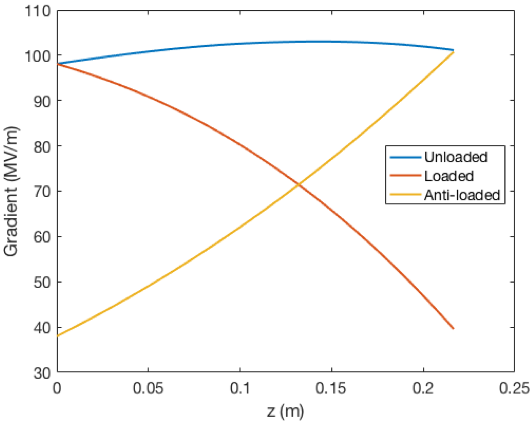
\includegraphics[scale=1]{pictures/3gradient.png}
\caption{Comparison of gradient profiles in different running conditions. The loaded and unloaded profiles are calculated at 43.3 MW input power, the antiloaded at 6.5 MW input power. The beam current in this case is 1.6 A.}
\label{3grad}
\end{figure}